% В рамках дипломной работы также был обнаружен способ улучшить этот фреймворк.

% Одна из упомянутых выше проблем - плохое покрытие тестами.
% В частности, результат получается нечитабельным, поскольку появляется внутреннее представление фреймворка, которое не является частью исходного кода.

% % // TODO: привести пример

% Этот недостаток можно устранить, если сжать генерируемые строки кода. 

% Еще одна вещь которую можно сделать - использовать вместо однострочных выражений с экранированием символов - многострочные.
% Результат, пускай и все еще тяжело воспринимается, значительно более читабелен чем ранее

% % // TODO: привести пример

% Уточнение про реализацию:
% более простым, а также более оптимальным решением было сделать сложный тег для открывающей и закрывающей скобки вместо того чтобы анализировать строки на наличие символов закрывающей кавычки и экранировать их.

% Еще одно улучшение было - добавить больше информации про локации оригинального кода для LSP.

% Рассматривался также вариант добавления каких-то указателей для bisect\_ppx, которые экранировали бы сгенерированный EML код.
% Однако, этот подход был исключен из рассмотрения по следующим причинам:
% \begin{itemize}
%     \item bisect\_ppx не имеет такой опции в принципе
%     \item результирующий код все еще должен быть компилируемым OCaml
%     \item метки также должны быть поддержаны LSP
% \end{itemize}

% Ни одно из этих ограничений не представляется возможным преодолеть, тем более все их вместе.

В результатах сравнения было выяснено что EML имеет плохую читабельность генерируемого кода.
В частности, результат получается нечитабельным, поскольку появляется внутреннее представление фреймворка, которое не является частью исходного кода.
Это внутреннее представление, однако, позволяет построить покрытие в целом и явно подсветить строки где код не покрыт.
Например, как видно на % // TODO: привести пример
В связи с этим, было принято решение не изменять эту функциональность.

Другая проблема заключается в том что весь HTML код шаблона сжимается в 1 строчку с экранированными символами.
Эту проблему можно решить, если использовать встроенный в OCaml\footnote{А также в Reason} синтаскис для многострочных строк.

Старая реализация опиралась на функцию \lstinline{Printf.kprintf} с модификатором \lstinline{%S}, которая экранирует символы и выводит их в генерируемый файл.
Вместо нее, в генерируемый файл будет выводиться строка как есть, заключенная в именованные кавычки
\lstinline{{___eml_tag|}
Имя кавычки необходимо в связи с ограничением синтаксиса многострочных литералов - текст внутри не может содержать последовательность символов |<tag>\}.
С этой проблемой можно было справиться другим способом - проверять код шаблона на наличие такой последовательности и экранировать ее в таком случае.
Однако это решение не является оптимальным, поскольку оно требует дополнительной проверки кода шаблона, а также сильно усложняет код парсера.
Потому более простое решение было выбрано.
Результат этой доработки можно посмотреть на рис. \ref{fig:improv}.

\begin{figure}[ht!]
    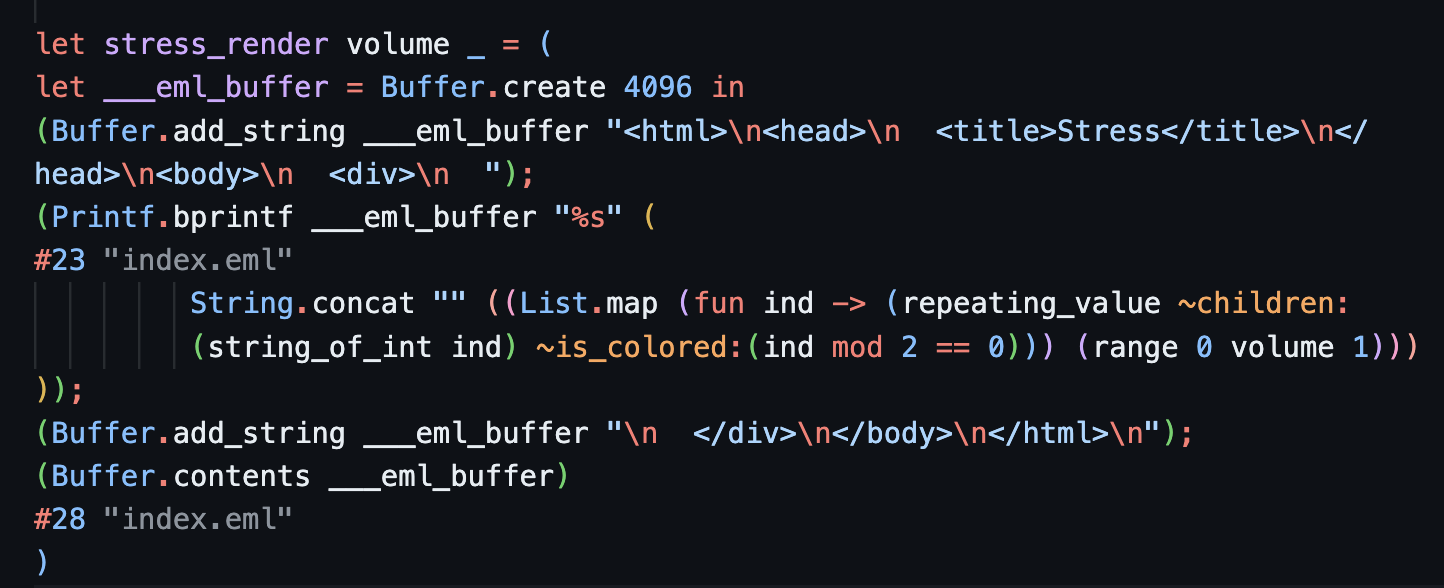
\includegraphics[width=.6\textwidth]{before}\hfill
    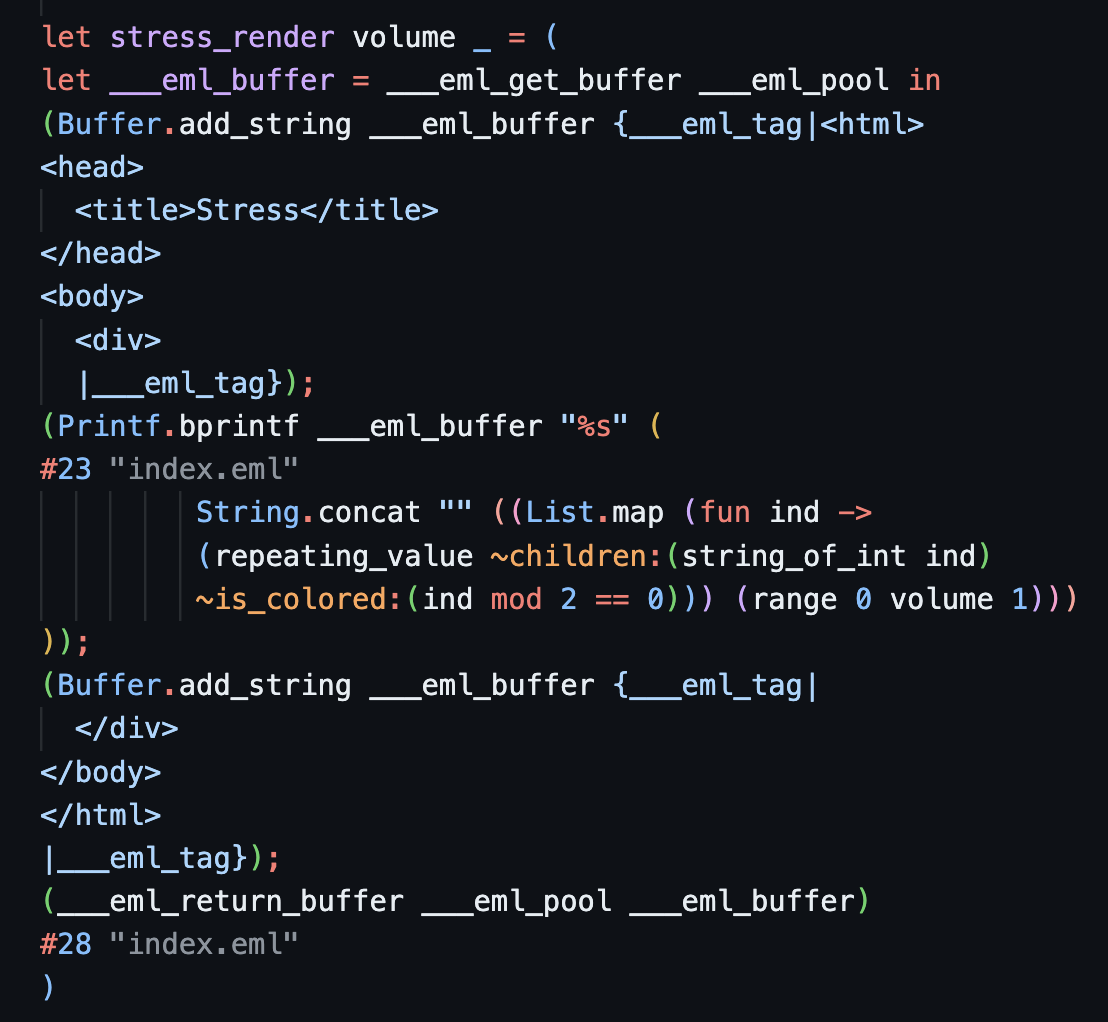
\includegraphics[width=.35\textwidth]{after}\hfill
    \caption{До изменений, код сжат в одну строчку}
    \caption{После изменений, код раздут в несколько строчек}
    \label{fig:improv}
\end{figure}
